% figures/foundations/system_layers.tex

\begin{figure}[ht]
\centering
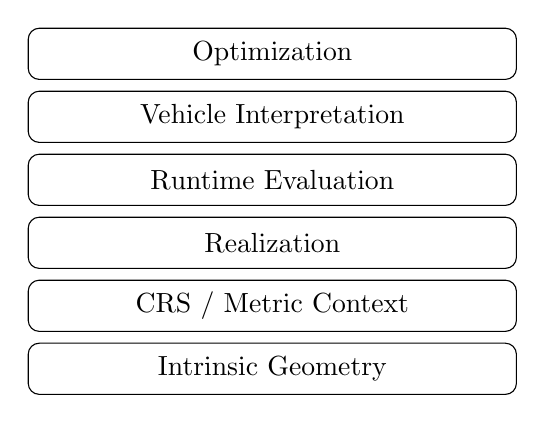
\begin{tikzpicture}[
  layer/.style={draw, rounded corners, align=center, minimum width=6.2cm, minimum height=0.65cm}
]
\node[layer] at (0,0) {Optimization};
\node[layer] at (0,-0.8) {Vehicle Interpretation};
\node[layer] at (0,-1.6) {Runtime Evaluation};
\node[layer] at (0,-2.4) {Realization};
\node[layer] at (0,-3.2) {CRS / Metric Context};
\node[layer] at (0,-4.0) {Intrinsic Geometry};
\end{tikzpicture}
\caption{AIM system layers: geometry is interpreted through metric, realization, runtime, vehicle, and optimization layers.}
\label{fig:system-layers}
\end{figure}
